\documentclass{llncs}
\usepackage{amsmath,amssymb,algorithm,algorithmic}
\usepackage{hyperref,color}
% No page numbers.
\usepackage{subfig}
\usepackage{graphicx}

\newcommand{\tool}{\text{ANTsR}}
\newcommand{\R}{{\bf R}}
\newcommand{\X}{{\bf X}}
\newcommand{\Xh}{{\hat{{\bf X}}}}
\newcommand{\x}{{\bf x}}
\newcommand{\Y}{{\bf Y}}
% \newcommand{\U}{{\bf U}}
\newcommand{\V}{{\bf V}}
\newcommand{\E}{{\bf E}}
\newcommand{\y}{{\bf y}}
\newcommand{\Z}{{\bf Z}}
\newcommand{\z}{{\bf z}}
\newcommand{\bSigma}{\boldsymbol \Sigma}
\newcommand{\vect}[1]{\mathbf{#1}}
\newcommand{\field}[1]{\mathbf{#1}}
\newcommand{\image}[1]{#1}
\newcommand{\I}{\image{I}}
\newcommand{\J}{\image{J}}
\renewcommand{\u}{\vect{u}}
\renewcommand{\v}{\vect{v}}
\renewcommand{\c}{\vect{c}}
\newcommand{\h}{\vect{h}}
\newcommand{\w}{\vect{w}}
\newcommand{\myphi}{\phi}
\newcommand{\mypsi}{\psi}
\newcommand{\D}{D}
\renewcommand{\d}{\nabla}
\newcommand{\dd}{\text{d}}
\newcommand{\p}{\partial}
\renewcommand{\L}{\Delta} % laplacian
\newcommand{\myS}{S}
\newcommand{\myR}{R}
\newcommand{\myE}{E}
\newcommand{\ld}{\langle}
\newcommand{\rd}{\rangle}
\newcommand{\LL}{\mathcal{L}} % operator L
\newcommand{\tQ}{\mathcal{Q}}
\newcommand{\Id}{\text{Id}}
\newcommand{\tG}{{G}} % operator L
\newcommand{\Diff}{\text{Diff}}
\newcommand{\VV}{\mathcal{V}}
\newcommand{\opL}{\mathcal{L}}
\newcommand{\bs}{\boldsymbol}
\newcommand{\tk}{~ITK$^{\text{4}}$~}
\newcommand{\bsp}{$\substack{
   \rightsquigarrow \\
   b
  }$}
\newcommand{\mi}{$\substack{
   \approx \\
   \text{mi}
  }$}
\newcommand{\cc}{$\substack{
   \approx \\
   \text{cc}
  }$}
\usepackage{setspace,verbatim}
\begin{document}
\vspace{-0.1in}
\title{Standardized Registration Methods for the SATA Challenge Datasets}
\author{Brian B. Avants$^1$, Nicholas J. Tustison$^2$, Hongzhi
  Wang$^1$ \\and the
  $^5$\href{http://www.insightsoftwareconsortium.org/}{Insight Software Consortium}\\
$^1$Penn Image Computing and Science Lab \\ Dept. of Radiology \\University of
  Pennsylvania, Philadelphia, PA, 19104\\ 
  $^2$Dept. of Radiology and Medical Imaging, \\ University of Virginia,
  Charlottesville, VA 22903\\
 $^5$\href{http://www.insightsoftwareconsortium.org/}{http://www.insightsoftwareconsortium.org/}}
\maketitle              
\begin{abstract}
The 2012 Segmentation: Algorithms, Theory and Applications (SATA)
challenge suggests that even subtle variation in registration
performance may impact the outcome of multi-atlas segmentation
algorithms. The 2013 SATA challenge organizers therefore requested
standardized registration that enables entrants to use the same
mappings as input to competing algorithms.  We therefore collaborated
to provide, within a relatively brief window of time, over 22,000
registration results based on Advanced Normalization Tools
(\href{http://stnava.github.io/ANTs/}{ANTs link}).
The diencephalon component of the challenge presented familiar and
easily addressed data requiring only 1,600 mappings between different
3D human T1 neuroimages.  The 3D multiple modality MRI ``dog leg'' dataset ($>$ 7,000
mappings) presented the opportunity to improve performance by using
a multivariate similarity metric.  The 4D cardiac (or CAP) dataset
($>$ 13,000 mappings) includes highly variable image quality, anatomy
and field of view.  We detail the ANTs variants that address the most basic brain dataset, where we used
a template-based approach, to the more challenging CAP dataset which
employed a more customized registration solution based on prior
knowledge.  The scripts, source code and a small set of example data
accompany this paper and are available online.  
\footnote{This work is supported by National Library of Medicine sponsored ARRA stimulus
funding.}
\end{abstract}

\begin{comment}
Brian,
 
One of the results of our multi-atlas workshop / challenge was that registration often had a larger impact on method performance than the statistical combination method (no real surprise there: garbage in = garbage out). SyN was used by the top two groups using Arno Klein’s published parameters.
 
In our journal write-up of the workshop results, we are planning on re-running the fusion algorithms using a common registration. Would you be willing to provide the “definitive” SyN results? We have 15 source images (plus label maps) that we need to match pair-wise to 20 target images (without label maps). If you would prefer to specify the command line parameters, Andrew (cc’d) can run the data through on our system.
 
Thanks!
Bennett

Dr. Avants,

After last year's MICCAI whole-brain segmentation challenge, two things became abundantly clear: (1) in order to isolate the benefits of specific label fusion algorithms we need to have a standardized registration and (2) the ANTs registration package represents the premier image registration framework. 

As a result, for this year's challenge (as part of the SATA workshop ) we would like to provide standardized atlas-target registrations for each of the datasets that we are considering.

Would you be willing to contribute these standardized registrations for the challenge?

The workshop website can be found here:
https://masi.vuse.vanderbilt.edu/workshop2013/index.php/Main_Page

The information on each of the datasets can be found here:
https://masi.vuse.vanderbilt.edu/workshop2013/index.php/Segmentation_Challenge_Details

The complete data package can be downloaded here:
https://masi.vuse.vanderbilt.edu/workshop2013/index.php/SATA_Data_Registration_Form

 For this year's challenge we are considering 3 datasets:
(1) A diencephalon (mid-brain) dataset
(2) A canine leg dataset
(3) A cardiac atlas dataset

From my perspective, I think that the mid-brain and canine leg datasets would not be terribly difficult to achieve consistent correspondence across the images. However, the cardiac atlas dataset might be significantly more challenging due to the way in which the images are acquired (i.e.,wildly varying orientations and fields-of-view).

We would greatly appreciate your help for making this challenge as successful as possible. If you have any questions/comments/concerns please do not hesitate to bring them up.

Thanks again,
Andrew Asman

\end{comment}

\section{Introduction}
Multi-atlas 
Using a common set of ``voters'' allows a more
direct comparison of the segmentation/fusion methods that are at the
heart of this challenge.   

``in order to isolate the benefits of specific label fusion algorithms we need to have a standardized registration''

The Insight ToolKit began a major refactoring effort in 2010.
The refactoring aimed to both simplify and extend the techniques available in version
3.x with methods and ideas from a new set of prior work
\cite{Jenkinson2001,Christensen1996,Rueckert1999,Miller2005,Peyrat2010,Avants2011}.
To make this technology more accessible, \tk unifies the dense
registration framework (displacement field, diffeomorphisms)
with the low-dimensional (B-Spline, Affine, rigid) framework by
introducing composite transforms, deformation field transforms and
specializations that allowed these to be optimized efficiently.  A sub-goal set for \tk was to simplify
parameter setting by adding helper methods that use well-known
principles of image registration to automatically scale transform
components and set optimization parameters.  \tk transforms are also
newly applicable to objects such as vectors and tensors and will take into account covariant geometry if
necessary.  Finally, \tk reconfigures the registration framework
to use multi-threading in as many locations as possible.
The revised registration framework within ITK is more thoroughly
integrated across transform models, is thread-safe and provides
broader functionality than in prior releases. 




\section{Challenge Data}
 For this year's challenge we are considering 3 datasets:
(1) A diencephalon (mid-brain) dataset
(2) A canine leg dataset
(3) A cardiac atlas dataset

From my perspective, I think that the mid-brain and canine leg datasets would not be terribly difficult to achieve consistent correspondence across the images. However, the cardiac atlas dataset might be significantly more challenging due to the way in which the images are acquired (i.e.,wildly varying orientations and fields-of-view).

\section{Methods}

\subsection{Diencephalon/Brain Data}

\subsection{Dog Leg Multi-Modality Data}

\subsection{CAP Cardiac Data}
\begin{figure}[t]
 \centering 
  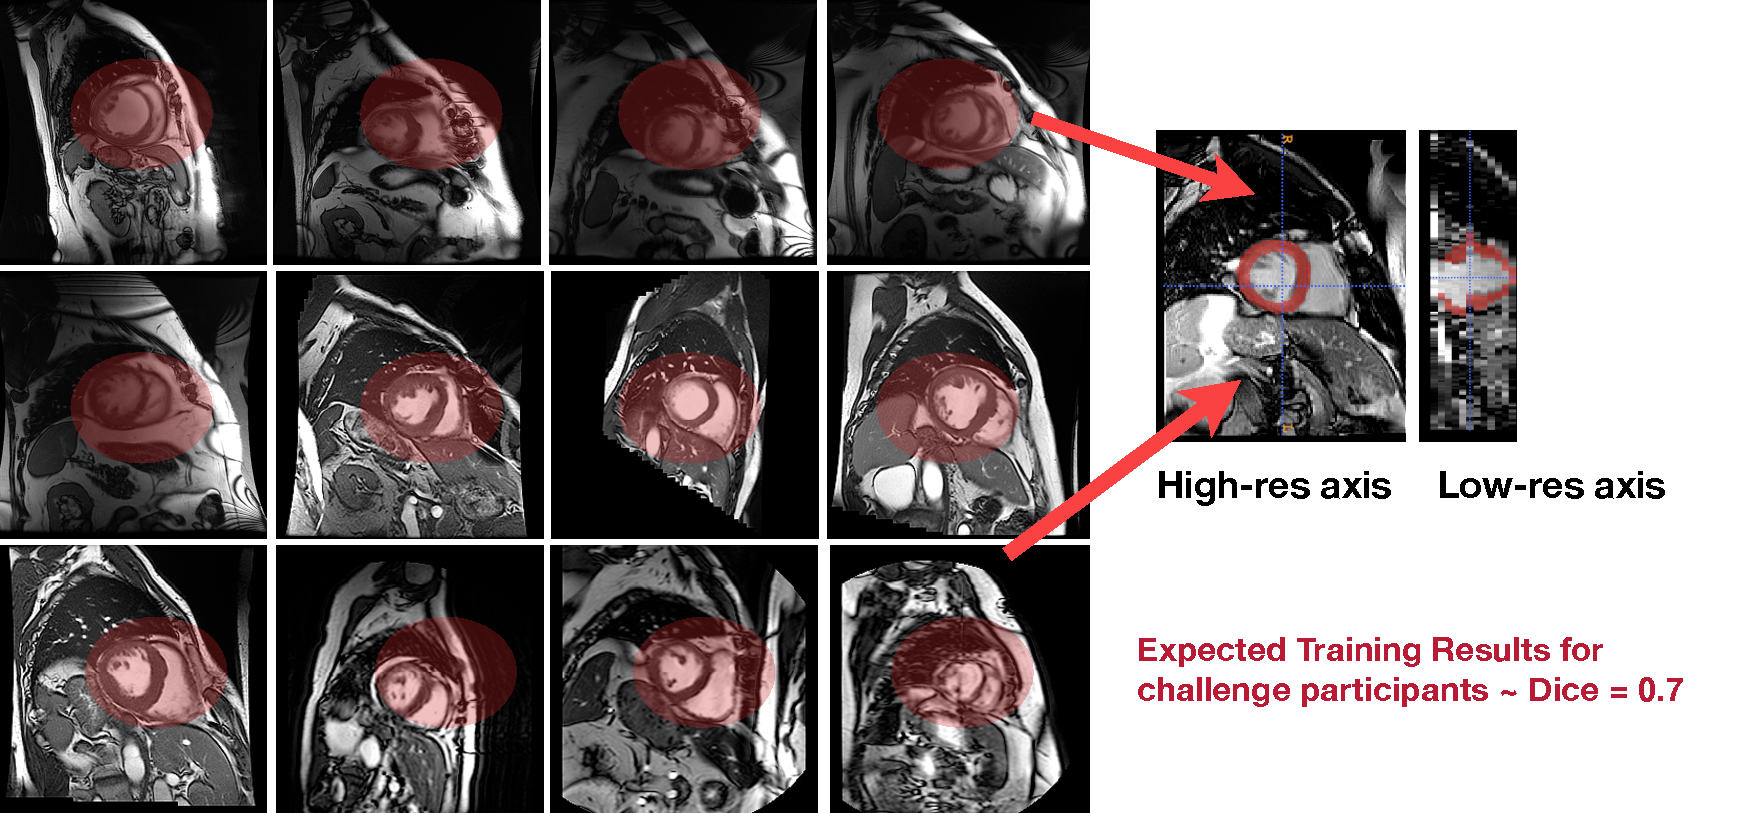
\includegraphics[width=5in]{../figs/CAP_methods.pdf}
 \caption{CAP methods}
 \label{fig:CAPmethods}
\end{figure}

\section{Results}

\subsection{Diencephalon/Brain Data}

\subsection{Dog Leg Multi-Modality Data}

\subsection{CAP Cardiac Data}
We estimated a failure rate of X\% on this data  .... look at
histogram of correlation 

\section{Discussion}

The cardiac dataset reveals some of the limitations involved with naive
pair-wise registration and highlights the benefit of
problem-specific strategies and multi-atlas methods.  

\bibliographystyle{splncs}
\bibliography{knobsock}
\end{document}

